%% =====================================================================
%%  Artigo cientifico - normas ABNT (classe abntex2)
%%  Sistema de reconhecimento mandibular digital
%%  Disciplina: Biomecanica - Engenharia Biomedica
%%
%%  COMPILACAO NO OVERLEAF:
%%    Menu > Settings > Compiler: pdfLaTeX
%%    Sequencia: pdfLaTeX -> BibTeX -> pdfLaTeX -> pdfLaTeX
%%    (o Overleaf faz isso automaticamente ao clicar em "Recompile")
%%
%%  ARQUIVOS NECESSARIOS: artigo.tex, referencias.bib, figuras/
%% =====================================================================

\documentclass[
    article,
    11pt,
    oneside,
    a4paper,
    english,
    brazil
]{abntex2}

% ----------------------------------------------------------------------
% Pacotes
% ----------------------------------------------------------------------
\usepackage[T1]{fontenc}
\usepackage[utf8]{inputenc}
\usepackage{lmodern}
\usepackage{indentfirst}
\usepackage{microtype}
\usepackage{graphicx}
\usepackage{booktabs}
\usepackage{multirow}
\usepackage{amsmath}
\usepackage{amssymb}
\usepackage{siunitx}
\usepackage{xcolor}
\usepackage{url}

% Citacoes ABNT NBR 10520 - sistema autor-data
\usepackage[alf]{abntex2cite}

% input-decimal-markers = {.,} permite digitar o numero com virgula OU com
% ponto. Sem essa linha, o siunitx v3 (versao atual do Overleaf) rejeita
% entradas como \num{0,525}. Nao remova.
\sisetup{
    input-decimal-markers = {.,},
    output-decimal-marker = {,},
    group-separator = {.},
    per-mode = symbol
}

\graphicspath{{figuras/}{../../resultados/}}

% ----------------------------------------------------------------------
% Informacoes de dados para folha de identificacao
% ----------------------------------------------------------------------
\titulo{Sistema de baixo custo para rastreamento do movimento mandibular
por visão computacional: desenvolvimento e demonstração de viabilidade
técnica}

\autor{Lívia Santelli Pegoraro\thanks{Graduanda em Engenharia Biomédica.
Matrícula 12321EBI010.} \and Maria Luisa Gonçalves
Ferreira\thanks{Graduanda em Engenharia Biomédica. Matrícula
12321EBI013.}}

\local{Brasil}
\data{2026}
\instituicao{Engenharia Biomédica --- Disciplina de Biomecânica}
\tipotrabalho{Artigo}

\preambulo{Artigo desenvolvido como atividade avaliativa da disciplina de
Biomecânica do curso de Engenharia Biomédica.}

% ----------------------------------------------------------------------
\begin{document}

\selectlanguage{brazil}
\frenchspacing

\maketitle

% ======================================================================
% RESUMO
% ======================================================================
\begin{resumoumacoluna}
A avaliação clínica do movimento mandibular é frequentemente conduzida por
inspeção visual, relato do paciente e mensuração manual com régua ou
paquímetro, procedimentos que dificultam a comparação objetiva entre
sessões de acompanhamento. Este trabalho descreve o desenvolvimento de um
sistema computacional de baixo custo para rastreamento do movimento
mandibular a partir de vídeo capturado por câmera comum. O sistema emprega
a biblioteca \textit{MediaPipe Face Landmarker} para localizar pontos
anatômicos faciais e calcula, em tempo real, três métricas
biomecânicas: abertura bucal, desvio lateral do mento e repetibilidade dos
ciclos de abertura e fechamento. Todas as distâncias são normalizadas pela
distância intercantal externa, tornando as medidas aproximadamente
invariantes à distância entre o rosto e a câmera. Foram implementados ainda
controle de qualidade por quadro, filtragem por média móvel exponencial,
detecção de ciclos por máquina de estados com histerese, biofeedback visual
e exportação de dados em formato aberto. Uma sessão de demonstração
(\num{1526} amostras, \SI{50,8}{\second}, \SI{30}{\hertz}) evidenciou
detecção estável dos marcadores em \SI{96}{\percent} dos quadros e
coeficiente de variação de \SI{3,2}{\percent} na amplitude de três ciclos
consecutivos de abertura máxima. Não foram realizadas comparação com método
de referência nem calibração em milímetros, de modo que os resultados
demonstram viabilidade técnica e repetibilidade interna, e não acurácia
metrológica. O sistema é apresentado como ferramenta de apoio didático e de
documentação funcional, não constituindo dispositivo médico nem substituindo
avaliação profissional.

\vspace{\onelineskip}

\noindent
\textbf{Palavras-chave}: biomecânica. articulação temporomandibular. visão
computacional. movimento mandibular. instrumentação de baixo custo.
\end{resumoumacoluna}

% ======================================================================
% ABSTRACT
% ======================================================================
\begin{resumoumacoluna}[Abstract]
\begin{otherlanguage*}{english}
Clinical assessment of mandibular movement is often carried out through
visual inspection, patient report and manual measurement with a ruler or
caliper, procedures that hinder objective comparison across follow-up
sessions. This work describes the development of a low-cost computational
system for tracking mandibular movement from video captured by an ordinary
webcam. The system employs the \textit{MediaPipe Face Landmarker} library to
locate facial anatomical points and computes, in real time, three
biomechanical metrics: mouth opening, lateral chin deviation and
repeatability of opening and closing cycles. All distances are normalised by
the outer intercanthal distance, making measurements approximately invariant
to the distance between face and camera. Per-frame quality control,
exponential moving average filtering, cycle detection by a hysteresis state
machine, visual biofeedback and open-format data export were also
implemented. A demonstration session (\num{1526} samples,
\SI{50.8}{\second}, \SI{30}{\hertz}) showed stable landmark detection in
\SI{96}{\percent} of frames and a coefficient of variation of
\SI{3.2}{\percent} in the amplitude of three consecutive maximum opening
cycles. Neither comparison against a reference method nor millimetre
calibration was performed, so results demonstrate technical feasibility and
internal repeatability rather than metrological accuracy. The system is
presented as a tool for educational support and functional documentation; it
is not a medical device and does not replace professional assessment.

\vspace{\onelineskip}

\noindent
\textbf{Keywords}: biomechanics. temporomandibular joint. computer vision.
mandibular movement. low-cost instrumentation.
\end{otherlanguage*}
\end{resumoumacoluna}

% ======================================================================
\textual

% ----------------------------------------------------------------------
\section{Introdução}
% ----------------------------------------------------------------------

A articulação temporomandibular (ATM) é a única articulação da cabeça
dotada de mobilidade ampla e funcionalmente relevante, servindo diretamente
à mastigação, à fonação e à deglutição \cite{dufour2016}. Alterações do
movimento mandibular podem manifestar-se como dor, redução de amplitude de
abertura, desvios laterais durante a trajetória e assimetria de movimento,
com repercussão direta em atividades cotidianas.

Na prática clínica, boa parte do acompanhamento dessas alterações apoia-se
em inspeção visual, relato do paciente e mensuração manual com régua ou
paquímetro. Tais procedimentos são de execução rápida e baixo custo, porém
apresentam duas limitações relevantes para o acompanhamento longitudinal:
registram apenas valores discretos, tipicamente a abertura máxima, sem
descrever a trajetória do movimento; e dependem da posição do instrumento e
do observador, o que introduz variabilidade entre sessões e entre
avaliadores.

Sistemas ópticos de captura de movimento e equipamentos de axiografia
oferecem medição detalhada da cinemática mandibular, mas seu custo e a
necessidade de ambiente controlado restringem seu emprego a contextos de
pesquisa. Entre esses dois extremos existe uma lacuna: instrumentos capazes
de registrar a trajetória do movimento de forma quantitativa, reprodutível e
exportável, mas viáveis em clínicas-escola e em atividades de ensino.

O desenvolvimento recente de bibliotecas de visão computacional capazes de
localizar pontos anatômicos faciais em tempo real a partir de vídeo
monocular, executáveis em hardware convencional
\cite{lugaresi2019,kartynnik2019}, torna possível abordar essa lacuna sem
instrumentação dedicada.

Este artigo tem por objetivo descrever o desenvolvimento de um sistema
computacional de baixo custo que, a partir de vídeo capturado por câmera
comum, rastreia o movimento mandibular e quantifica abertura bucal, desvio
lateral do mento e repetibilidade dos ciclos de abertura e fechamento. São
objetivos específicos: (i) definir métricas biomecânicas normalizadas e
independentes da distância entre o rosto e a câmera; (ii) implementar
controle de qualidade, filtragem e detecção automática de ciclos;
(iii) prover biofeedback visual e exportação de dados em formato aberto; e
(iv) demonstrar a viabilidade técnica do sistema em uma sessão de coleta.

Delimita-se, desde já, o alcance do trabalho: trata-se de ferramenta de
apoio e de uso didático. O sistema não constitui dispositivo médico, não
emite diagnóstico e não substitui a avaliação de profissional habilitado.

% ----------------------------------------------------------------------
\section{Fundamentação teórica}
% ----------------------------------------------------------------------

\subsection{Anatomia funcional da articulação temporomandibular}

A ATM é classificada anatomicamente como articulação bicondilar: há duas
articulações, direita e esquerda, fisicamente separadas, mas
funcionalmente acopladas, de modo que o movimento de uma condiciona o da
outra \cite{dufour2016}. As superfícies articulares compreendem, no crânio,
o tubérculo articular do temporal e a fossa mandibular e, na mandíbula, o
côndilo mandibular. Interpõe-se entre elas o disco articular, menisco móvel
que recobre o côndilo e divide a cavidade em compartimentos superior e
inferior, sendo tracionado anteriormente pelo músculo pterigóideo lateral
durante a abertura da boca \cite{dufour2016}.

A posição de estabilidade passiva corresponde ao fechamento da boca com os
dentes engrenados; a abertura máxima é estabilizada ativamente pela
musculatura. As posições intermediárias configuram a condição de maior
exigência mecânica, quando o movimento de propulsão se soma ao de
abaixamento \cite{dufour2016}. Essa característica justifica o interesse em
registrar a \textit{trajetória} completa do movimento, e não apenas seus
valores extremos.

\subsection{Movimentos mandibulares e amplitudes de referência}

A mobilidade da ATM pode ser descrita por movimentos analíticos elementares
e por sua combinação funcional \cite{dufour2016}:

\begin{alineas}
    \item \textbf{abaixamento--elevação}: movimento sagital em torno de eixo
    transversal que passa pelo centro das cabeças condilares, correspondente
    à abertura angular pura;
    \item \textbf{propulsão--retropulsão}: deslizamento anteroposterior em
    plano horizontal, com amplitude normal de \SIrange{6}{8}{\milli\metre}
    medida entre os incisivos;
    \item \textbf{didução}: lateralização da ponta do mento, produzida pelo
    avanço unilateral de um côndilo enquanto o contralateral permanece na
    fossa, com amplitude média de \SIrange{9}{12}{\milli\metre};
    \item \textbf{abertura da boca}: mobilidade funcional resultante da
    combinação de abaixamento angular, até cerca de
    \SI{20}{\milli\metre} de afastamento dentário, ao qual se associa em
    seguida a propulsão, com amplitude normal média de
    \SIrange{40}{60}{\milli\metre}.
\end{alineas}

As faixas de \SIrange{40}{60}{\milli\metre} para abertura e de
\SIrange{9}{12}{\milli\metre} para didução constituem as referências
adotadas neste trabalho para contextualização das medidas
\cite{dufour2016}. Cabe registrar que sua aplicação exige calibração de
escala, conforme discutido na Seção~\ref{sec:calibracao}.

\subsection{Assimetria facial e ausência de limiar de referência}
\label{sec:assimetria}

Diferentemente das amplitudes de movimento, a assimetria facial não dispõe,
na literatura consultada, de limiar quantitativo que separe a condição
fisiológica da patológica. As fontes examinadas convergem na afirmação de
que a assimetria é característica universal das faces humanas, sem
estabelecer valor de corte em milímetros ou pontos percentuais. Essa
constatação orientou uma decisão de projeto deliberada: o índice de
simetria calculado pelo sistema é apresentado exclusivamente como parâmetro
de comparação intrassujeito, de caráter didático, sem classificação
clínica associada. A implicação metodológica é discutida na
Seção~\ref{sec:discussao}.

% ----------------------------------------------------------------------
\section{Materiais e métodos}
% ----------------------------------------------------------------------

\subsection{Arquitetura do sistema}

O sistema foi implementado em linguagem Python, organizado em módulos de
responsabilidade única. A camada de aquisição e apresentação utiliza a
biblioteca OpenCV \cite{bradski2000}; a localização dos pontos anatômicos
faciais emprega o modelo \textit{Face Landmarker} da biblioteca MediaPipe
\cite{lugaresi2019}, que estima em tempo real uma malha densa de vértices
sobre a face a partir de vídeo monocular \cite{kartynnik2019}.

O fluxo de processamento, executado a cada quadro, compreende seis etapas:
aquisição da imagem; localização dos marcadores faciais; avaliação da
qualidade do quadro; cálculo das métricas biomecânicas; filtragem temporal;
e atualização do detector de ciclos, do biofeedback e do registro de dados.
A separação entre a lógica de desenho e a lógica de cálculo permitiu
reutilizar o mesmo código de sobreposição gráfica nos modos de operação ao
vivo e de reprocessamento de vídeo gravado.

\subsection{Definição do referencial facial}

Para tornar as medidas robustas à rotação da cabeça no plano da imagem,
construiu-se um referencial local solidário à face. Sejam
$\mathbf{p}_{oe}$ e $\mathbf{p}_{od}$ as posições dos cantos externos dos
olhos esquerdo e direito, em pixels. Definem-se o versor horizontal e o
versor vertical da face por

\begin{equation}
    \hat{\mathbf{x}}_{f} =
        \frac{\mathbf{p}_{od} - \mathbf{p}_{oe}}
             {\lVert \mathbf{p}_{od} - \mathbf{p}_{oe} \rVert},
    \qquad
    \hat{\mathbf{y}}_{f} =
        \begin{bmatrix} -\hat{x}_{f,y} \\ \hat{x}_{f,x} \end{bmatrix},
    \label{eq:referencial}
\end{equation}

\noindent
sendo $\hat{\mathbf{y}}_{f}$ perpendicular a $\hat{\mathbf{x}}_{f}$ e
orientado para baixo na imagem. Adota-se como referência de escala a
distância intercantal externa

\begin{equation}
    L_{f} = \lVert \mathbf{p}_{od} - \mathbf{p}_{oe} \rVert ,
    \label{eq:largura}
\end{equation}

\noindent
grandeza escolhida por não se alterar com a abertura da boca, ao contrário
de referências como a largura labial.

\subsection{Métricas biomecânicas}

\subsubsection{Abertura bucal}

A abertura bucal é obtida como a projeção, sobre o eixo vertical da face, do
vetor que une os pontos labiais internos superior ($\mathbf{p}_{ls}$) e
inferior ($\mathbf{p}_{li}$), normalizada pela referência de escala:

\begin{equation}
    A_{rel} =
        \frac{\lvert (\mathbf{p}_{li} - \mathbf{p}_{ls}) \cdot
              \hat{\mathbf{y}}_{f} \rvert}{L_{f}} .
    \label{eq:abertura}
\end{equation}

\subsubsection{Desvio lateral do mento}

O desvio lateral é obtido como a projeção, sobre o eixo horizontal da face,
do vetor que une a raiz do nariz ($\mathbf{p}_{n}$), ponto próximo da linha
média, à ponta do mento ($\mathbf{p}_{m}$):

\begin{equation}
    D_{rel} =
        \frac{(\mathbf{p}_{m} - \mathbf{p}_{n}) \cdot
              \hat{\mathbf{x}}_{f}}{L_{f}} .
    \label{eq:desvio}
\end{equation}

A grandeza preserva o sinal, o que permite distinguir o lado do desvio. A
tradução do sinal em rótulo textual considera o espelhamento da imagem:
quando a imagem é exibida espelhada, condição adotada por padrão para
proporcionar experiência de espelho ao usuário, o semieixo positivo
corresponde ao lado direito do próprio paciente; sem espelhamento, essa
relação se inverte. A ausência dessa correção produziria rótulo invertido
sempre que o espelhamento fosse desativado.

\subsubsection{Repetibilidade dos ciclos}

A detecção de ciclos de abertura e fechamento foi implementada por máquina
de estados com quatro estados --- fechado, abrindo, aberto e fechando ---
cujas transições empregam dois limiares distintos, configurando histerese.
O emprego de limiares separados para abertura e para fechamento evita
contagens espúrias decorrentes de oscilação do sinal em torno de um único
valor de corte. Para cada ciclo completo registram-se amplitude e duração;
ao conjunto de ciclos de uma sessão calcula-se o coeficiente de variação da
amplitude,

\begin{equation}
    CV = \frac{\sigma_{A}}{\bar{A}} ,
    \label{eq:cv}
\end{equation}

\noindent
adotado como indicador de repetibilidade intrassessão.

\subsection{Calibração de escala}
\label{sec:calibracao}

As métricas definidas nas Equações~\eqref{eq:abertura} e~\eqref{eq:desvio}
são adimensionais, expressas em unidades de largura facial. A conversão para
milímetros é opcional e requer a informação da distância intercantal externa
real do indivíduo, $L_{mm}$, fornecida por parâmetro de execução. Nesse
caso, obtém-se $A_{mm} = A_{rel} \cdot L_{mm}$, e analogamente para o desvio
lateral.

Duas ressalvas são relevantes. Primeira: a conversão é uma
\textit{estimativa}, cuja incerteza depende da medição de $L_{mm}$ e do
posicionamento da cabeça. Segunda: a calibração dos limiares funcionais da
máquina de estados é sempre realizada na escala relativa, de modo
independente da conversão métrica, o que permite operar o sistema sem
calibração dimensional quando o interesse recai sobre a trajetória e a
repetibilidade, e não sobre o valor absoluto.

Para apoiar a definição dos limiares, implementou-se assistente de
calibração que conduz o usuário por duas posturas de referência, boca
fechada e boca aberta, registrando os valores correspondentes de
$A_{rel}$.

\subsection{Controle de qualidade e filtragem}

Cada quadro é classificado em três categorias --- não detectado, inválido ou
válido --- a partir de critérios de tamanho relativo do rosto, inclinação da
cabeça e magnitude do deslocamento entre quadros consecutivos. Quadros
inválidos são excluídos do cálculo das métricas e da contagem de ciclos,
evitando que ruído de detecção contamine os resultados.

O tamanho do rosto é avaliado pela razão entre a largura facial em pixels e
a largura do quadro, $L_{f}/W$, e não pela diagonal da imagem. A razão
adotada permanece constante para uma mesma distância real entre rosto e
câmera, independentemente da resolução de captura, propriedade que a razão
pela diagonal não apresenta.

Os sinais de abertura, desvio lateral e largura facial são suavizados por
média móvel exponencial,

\begin{equation}
    s_{k} = \alpha \, x_{k} + (1 - \alpha)\, s_{k-1} ,
    \label{eq:ema}
\end{equation}

\noindent
com coeficiente $\alpha$ ajustado independentemente para cada sinal. O filtro
foi escolhido por reduzir o ruído de localização dos marcadores quadro a
quadro sem introduzir o atraso perceptível associado a médias móveis de
janela larga, requisito imposto pela apresentação do biofeedback em tempo
real.

\subsection{Biofeedback e exportação de dados}

A interface apresenta, sobrepostos à imagem ao vivo, os marcadores
anatômicos, uma barra indicadora da abertura, painel com os valores
instantâneos e o estado corrente do movimento. As mensagens de orientação
descrevem exclusivamente o observado --- posicionamento, faixa de abertura,
sentido do desvio, regularidade das repetições --- sem emitir julgamento
clínico ou sugestão diagnóstica.

Cada sessão é exportada em diretório próprio, contendo a série temporal
completa em formato CSV, resumo estatístico, metadados de execução e
gráficos da evolução temporal. A identificação é anônima por padrão,
composta apenas por data e hora da coleta.

\subsection{Protocolo de coleta e sessão de demonstração}

O protocolo estabelece iluminação difusa e suficiente, rosto centralizado no
quadro, cabeça estável e ausência de rotação acentuada fora do plano da
imagem. Ao usuário solicita-se a execução de ciclos completos de abertura e
fechamento máximos, sem lateralização voluntária.

Para demonstrar a viabilidade técnica do sistema, analisou-se uma sessão
registrada em \SI{30}{\hertz} com câmera de computador pessoal. Os dados
correspondem a um único indivíduo adulto, integrante da equipe de
desenvolvimento, e foram coletados sem calibração dimensional. O trecho
exportado compreende \num{1526} amostras ao longo de \SI{50,8}{\second}.
Ressalva-se que se trata de coleta de caráter técnico, destinada a verificar
o funcionamento do sistema, e não de estudo com amostra populacional.

% ----------------------------------------------------------------------
\section{Resultados}
% ----------------------------------------------------------------------

\subsection{Estabilidade da detecção}

Dos \num{1526} quadros processados, \num{1465} foram classificados como
frontais válidos, correspondendo a \SI{96}{\percent} do total. A taxa média
de amostragem efetiva foi de \SI{30,0}{\hertz}, com intervalo mediano entre
amostras de \SI{32,9}{\milli\second}, compatível com a operação em tempo
real pretendida.

\subsection{Métricas do movimento}

A Tabela~\ref{tab:metricas} apresenta a estatística descritiva das métricas
registradas na sessão. Os valores de abertura e desvio lateral são
expressos em unidades de largura facial, uma vez que a sessão foi conduzida
sem calibração dimensional.

\begin{table}[htb]
    \centering
    \caption{Estatística descritiva das métricas na sessão de demonstração
    ($n = \num{1526}$ amostras; \SI{50,8}{\second}).}
    \label{tab:metricas}
    \begin{tabular}{lrrrr}
        \toprule
        \textbf{Métrica} & \textbf{Média} & \textbf{DP} &
        \textbf{Mín.} & \textbf{Máx.} \\
        \midrule
        Abertura bucal [larg. facial]     & 0,059 & 0,133 & 0,000 & 0,525 \\
        Desvio lateral [larg. facial]     & 0,023 & 0,009 & $-$0,030 & 0,091 \\
        Índice de simetria [0--1]         & 0,858 & 0,151 & 0,000 & 0,967 \\
        Desvio da linha média [larg. fac.]& $-$0,001 & 0,019 & $-$0,168 & 0,024 \\
        Inclinação (\textit{cant}) [\si{\degree}] & $-$0,34 & 0,88 & $-$6,54 & 1,93 \\
        Razão dos terços faciais          & 0,969 & 0,103 & 0,622 & 1,247 \\
        Razão dos quintos faciais         & 4,781 & 0,119 & 4,130 & 5,134 \\
        Razão intercantal/alar            & 0,894 & 0,050 & 0,735 & 1,059 \\
        \bottomrule
    \end{tabular}
    \par\vspace{0.3cm}
    \footnotesize
    Fonte: dados da pesquisa. DP: desvio-padrão populacional.
\end{table}

A distribuição temporal dos estados do movimento indicou predominância do
estado fechado, presente em \SI{91,3}{\percent} das amostras, seguido do
estado aberto, em \SI{8,3}{\percent}; os estados de transição, abrindo e
fechando, somaram \SI{0,4}{\percent}. Essa proporção é coerente com o
protocolo, em que os ciclos de abertura máxima são intercalados por
intervalos de repouso.

\subsection{Repetibilidade}

No trecho analisado, o detector registrou três ciclos completos de abertura
e fechamento, com amplitudes de \num{0,525}, \num{0,508} e \num{0,485}
unidades de largura facial. O coeficiente de variação da amplitude, obtido
pela Equação~\eqref{eq:cv}, resultou em \SI{3,2}{\percent}.

Cabe registrar que o contador cumulativo de repetições iniciava em 62 no
primeiro quadro do arquivo exportado, indicando que o trecho analisado
corresponde ao segmento final de uma sessão mais longa. As amplitudes foram
obtidas por segmentação \textit{a posteriori} da série temporal com base nas
transições do contador.

\subsection{Registro gráfico}

A Figura~\ref{fig:evolucao} reproduz o gráfico gerado automaticamente pelo
sistema ao término da sessão. No painel superior, os três ciclos de abertura
máxima aparecem como platôs próximos a \num{0,50} unidades de largura
facial, entre \SI{177}{\second} e \SI{186}{\second}, delimitados pelas
linhas verticais tracejadas que marcam os ciclos detectados. Os eventos de
menor amplitude observados após \SI{190}{\second} não foram contabilizados
como ciclos, por não atingirem o limiar de abertura configurado.

\begin{figure}[htb]
    \centering
    \caption{Evolução temporal da abertura bucal, do desvio lateral do mento
    e do índice de simetria durante a sessão de demonstração.}
    \label{fig:evolucao}
    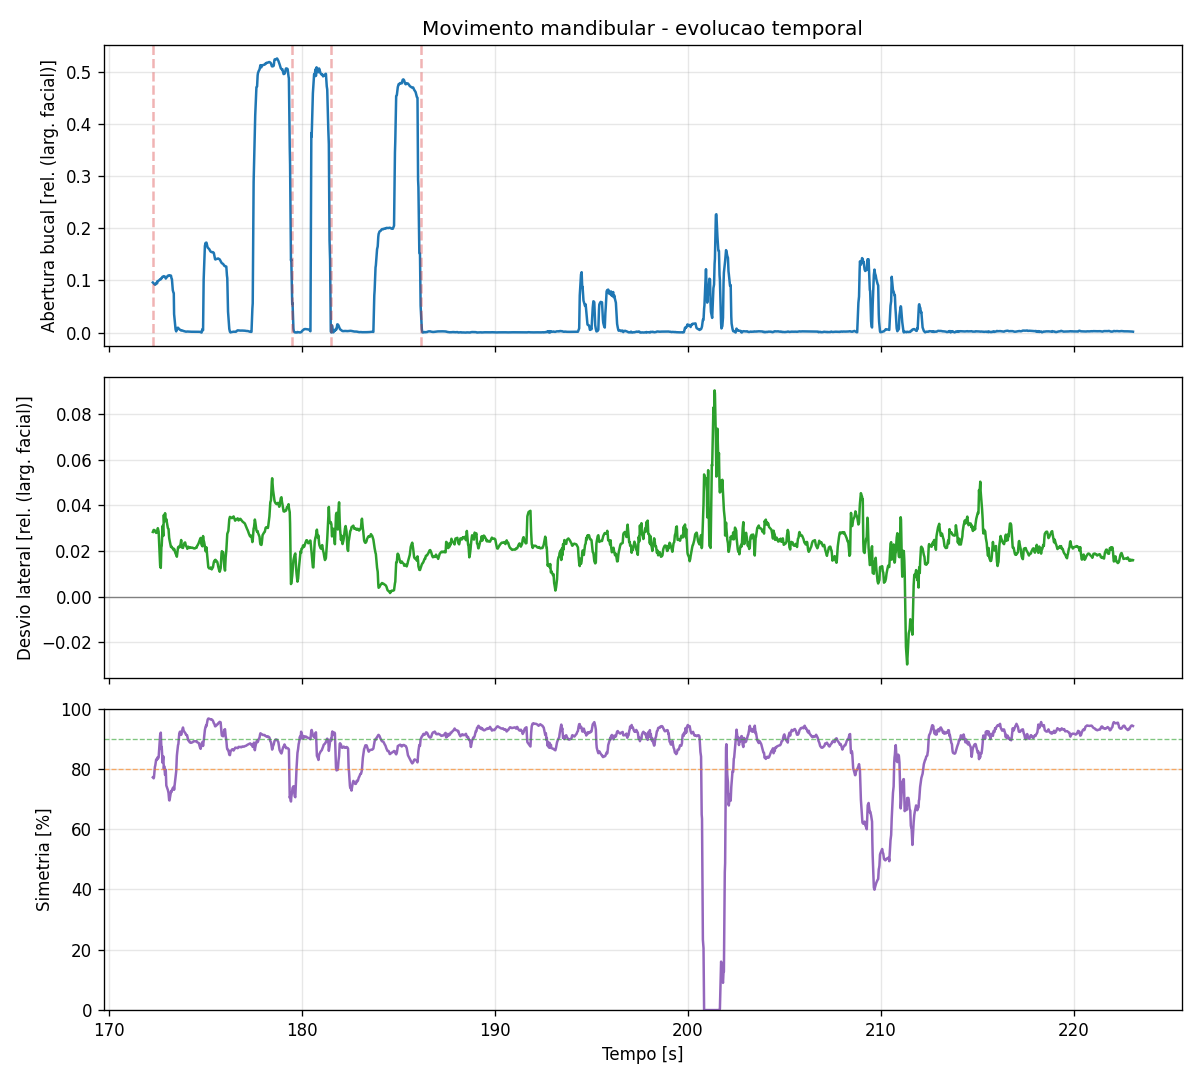
\includegraphics[width=\textwidth]{sessao_20260724_142153.png}
    \par\vspace{0.2cm}
    \footnotesize
    Fonte: saída gráfica gerada pelo sistema desenvolvido.
\end{figure}

O painel intermediário mostra o desvio lateral oscilando em torno de
\num{0,023} unidades de largura facial, com excursão máxima de \num{0,091}
em torno de \SI{201}{\second}. O painel inferior apresenta o índice de
simetria, majoritariamente contido entre \SI{80}{\percent} e
\SI{95}{\percent}, com queda abrupta a zero no intervalo de
\SI{200,5}{\second} a \SI{202}{\second}. Essa descontinuidade é analisada na
Seção~\ref{sec:discussao}.

% ----------------------------------------------------------------------
\section{Discussão}
\label{sec:discussao}
% ----------------------------------------------------------------------

Os resultados indicam que a localização de marcadores faciais por vídeo
monocular, associada à normalização pela distância intercantal externa,
permite registrar a trajetória do movimento mandibular com estabilidade
suficiente para acompanhamento funcional. A detecção válida em
\SI{96}{\percent} dos quadros e a taxa efetiva de \SI{30}{\hertz} atendem ao
requisito de operação em tempo real, e o coeficiente de variação de
\SI{3,2}{\percent} na amplitude de ciclos consecutivos sugere
repetibilidade intrassessão adequada ao propósito de comparação entre
repetições.

Três limitações delimitam a interpretação desses achados.

A primeira e mais relevante é a ausência de comparação com método de
referência. Não foram realizadas medições concomitantes com paquímetro ou
com sistema óptico de captura de movimento. Consequentemente, os resultados
sustentam afirmações sobre \textit{repetibilidade} --- a capacidade de o
sistema produzir valores semelhantes em repetições semelhantes --- mas não
sobre \textit{acurácia}, isto é, a proximidade entre o valor medido e o
valor verdadeiro. Nenhuma conclusão sobre validade metrológica pode ser
extraída deste trabalho.

A segunda decorre da ausência de calibração dimensional na sessão
analisada. Sem a informação da distância intercantal real, as medidas
permanecem em unidades de largura facial e não podem ser confrontadas com as
faixas de \SIrange{40}{60}{\milli\metre} para abertura e
\SIrange{9}{12}{\milli\metre} para didução. A comparação com essas
referências, ainda que o sistema a suporte, permanece como etapa não
executada.

A terceira refere-se à amostra: um único indivíduo, uma única sessão. Não
há, portanto, base para afirmações sobre desempenho em diferentes tipos
faciais, faixas etárias ou condições clínicas.

A descontinuidade observada no índice de simetria, com queda a zero entre
\SI{200,5}{\second} e \SI{202}{\second}, ilustra concretamente uma
vulnerabilidade do método. O valor nulo não representa achado
biomecânico, mas falha momentânea de localização dos marcadores,
provavelmente associada a rotação da cabeça fora do plano da imagem ou a
oclusão parcial da face. O episódio demonstra a necessidade do controle de
qualidade por quadro e indica, como aperfeiçoamento, a propagação explícita
da condição de dado ausente para as séries exportadas, em vez do registro de
valor numérico nulo.

Merece registro, ainda, a decisão relativa ao índice de simetria discutida
na Seção~\ref{sec:assimetria}. Diante da constatação de que a literatura
consultada não fornece limiar que distinga assimetria fisiológica de
patológica, optou-se por não estabelecer classificação clínica para essa
métrica, mantendo-a como parâmetro de comparação intrassujeito. A alternativa
--- adotar um valor de corte arbitrário --- produziria saída de aparência
clínica sem fundamentação, risco especialmente relevante em ferramenta
destinada a contexto de ensino. A mesma orientação foi aplicada às demais
métricas: cada classificação emitida pelo sistema é acompanhada da fonte do
valor de referência e de ressalva explícita quanto ao seu caráter de apoio.

Como perspectivas de continuidade, identificam-se: a validação concorrente
contra paquímetro digital em amostra com múltiplos participantes; a
estimação da pose tridimensional da cabeça para compensar rotações fora do
plano; e a avaliação da concordância entre sessões, com vistas ao emprego do
histórico de evolução já implementado.

% ----------------------------------------------------------------------
\section{Considerações finais}
% ----------------------------------------------------------------------

Este trabalho descreveu o desenvolvimento de um sistema de baixo custo para
rastreamento do movimento mandibular por visão computacional, operando com
câmera comum e bibliotecas de uso livre. Foram implementadas métricas
biomecânicas normalizadas de abertura bucal, desvio lateral do mento e
repetibilidade de ciclos, além de controle de qualidade por quadro,
filtragem temporal, detecção automática de ciclos, biofeedback visual e
exportação de dados em formato aberto.

A sessão de demonstração evidenciou detecção estável em \SI{96}{\percent}
dos quadros, operação a \SI{30}{\hertz} e coeficiente de variação de
\SI{3,2}{\percent} na amplitude de três ciclos consecutivos, resultados que
sustentam a viabilidade técnica da abordagem. Não tendo sido realizadas
calibração dimensional nem comparação com método de referência, os achados
não autorizam afirmações sobre acurácia metrológica.

A contribuição do trabalho reside menos no desempenho numérico alcançado e
mais na demonstração de que imagens obtidas por equipamento comum podem ser
convertidas em informação quantitativa, reprodutível e documentável sobre o
movimento mandibular, com potencial de emprego no ensino de biomecânica e no
registro da evolução funcional. Reitera-se que o sistema constitui
ferramenta de apoio e de uso didático, não sendo dispositivo médico nem
substituto da avaliação de profissional habilitado.

% ======================================================================
\bibliography{referencias}

\end{document}
